% Tikz File 'SWE.tex'
\documentclass{standalone}
\usepackage{tikz}
\usetikzlibrary {arrows.meta} 
\begin{document}
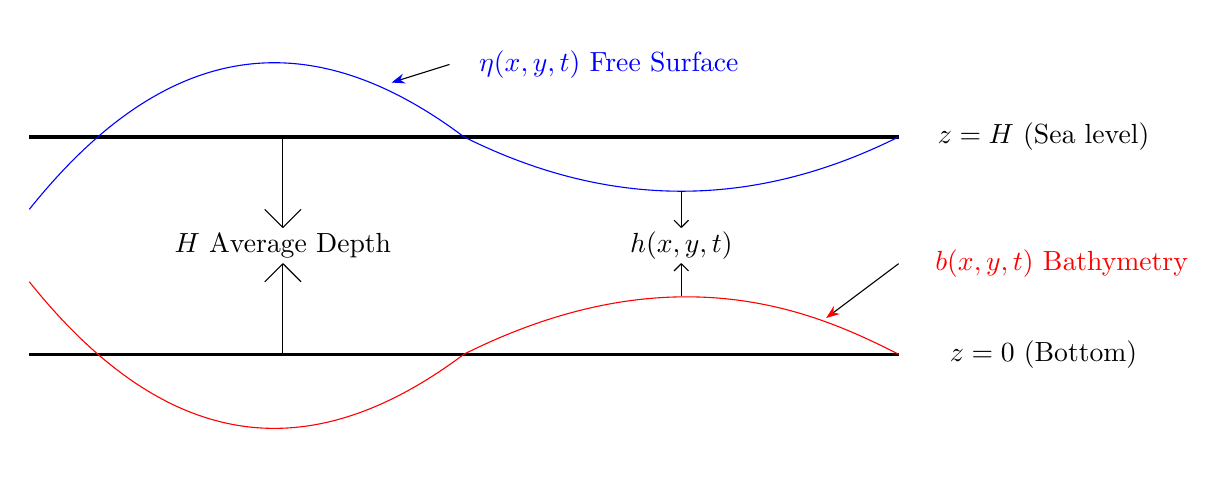
\begin{tikzpicture}[scale=0.46]
		\draw[very thick] (-12,0) -- (12,0);
		\draw[very thick] (-12,6) -- (12,6);
		\draw[red] (-12,2) .. controls (-8,-3) and (-4,-3) .. (0,0);
		\draw[red] (0,0) .. controls (6,3) and (10,1) .. (12,0);
		\draw[blue] (-12,4) .. controls (-8,9) and (-4,9) .. (0,6);
		\draw[blue] (0,6) .. controls (4,4) and (8,4) .. (12,6);
		\node at (16,6) {$z=H$ (Sea level)};
		\node at (16,0) {$z=0$ (Bottom)};
		\draw[-{Stealth[blue]}] (-0.4,8)   -- (-2,7.5);
		\node[blue] at (4,8) {$\eta(x,y,t)$ Free Surface};
		\draw[-{Stealth[red]}] (12,2.5)   -- (10,1);
		\node[red] at (16.5,2.5) {$b(x,y,t)$ Bathymetry};
		\draw(6,4.5) -- (6,3.5);
		\draw(5.8,3.7) -- (6,3.5);
        \draw(6.2,3.7) -- (6,3.5);
		\draw(6,1.6) -- (6,2.5);
        \draw(6,2.5) -- (5.8,2.3);
        \draw(6.2,2.3)--(6,2.5);
		\node at (6,3) {$h(x,y,t)$};
		\draw(-5,6) -- (-5,3.5);
		\draw(-5.5,4.0) -- (-5,3.5);
        \draw(-5,3.5) -- (-4.5,4.0);
		\draw(-5,2.5) -- (-5.5,2);
        \draw(-5,2.5) -- (-4.5,2);
		\draw(-5,0) -- (-5,2.5);
		\node at (-5,3) {$H$ Average Depth};
	\end{tikzpicture}
\end{document}